\chapter{Réalisation du dispositif}
\section{Introduction}
Pour réaliser le dispositif destiné à une installation de 12 kW et 400 V, nous avons rencontré des défis liés à la disponibilité des batteries et des capteurs nécessaires pour atteindre ces spécifications. Par conséquent, nous avons choisi de simuler le système à une échelle réduite en utilisant une installation domestique. Cette approche nous permet de tester les principes et le fonctionnement du système tout en réduisant le nombre de capteurs et de batteries à surveiller.

Les composants et le fonctionnement du dispositif à petite échelle sont identiques à ceux du système prévu pour 12 kW, garantissant ainsi que les résultats obtenus peuvent être extrapolés à une plus grande échelle. Cette méthode nous permet de valider le concept, d'optimiser le design, et de résoudre d'éventuels problèmes avant de passer à une installation plus importante.

\subsection{Conception et dimensionnement des divers composants du système}
L'interface de puissance dans ce projet joue un rôle crucial en gérant les interactions entre les éléments de contrôle à basse tension (comme l'ESP32) et les composants de puissance plus élevés, tels que les batteries et les relais. Elle permet d'assurer une protection efficace des composants sensibles tout en maintenant un contrôle précis des charges et de la mesure des courants, tensions et températures dans le système.

\subsubsection{Circuits de l’interface de puissance}

Le système de surveillance intègre plusieurs circuits de puissance pour gérer la charge, la décharge et la mesure des paramètres des batteries. Les relais 5V DC sont pilotés par des transistors 2N2222, car les broches de l'ESP32 ne fournissent que du 3.3V, alors que la tension d'activation des relais est de 5V. Pour la mesure de tension, des diviseurs de tension équipés de diodes Zener 1N4728A sont utilisés afin de réduire la tension et protéger les entrées du microcontrôleur. En ce qui concerne la mesure de courant, les capteurs ACS712 sont également reliés à des diviseurs de tension pour adapter la tension de sortie à un niveau acceptable pour l'ESP32.

\subsubsection*{Module relais et transistor 2N2222}

Les modules relais permettent de contrôler des charges électriques importantes en réponse aux commandes de l'ESP32. Étant donné que les sorties de l'ESP32 ne délivrent que 3.3V, des transistors 2N2222 sont utilisés comme commutateurs pour activer les relais 5V. Cette configuration permet de commuter des charges plus élevées tout en protégeant le microcontrôleur des courants et tensions élevés.

\subsubsection*{Calcul de la Résistance de Base (\(R_B\))}


\begin{figure}[H]
	\centering
	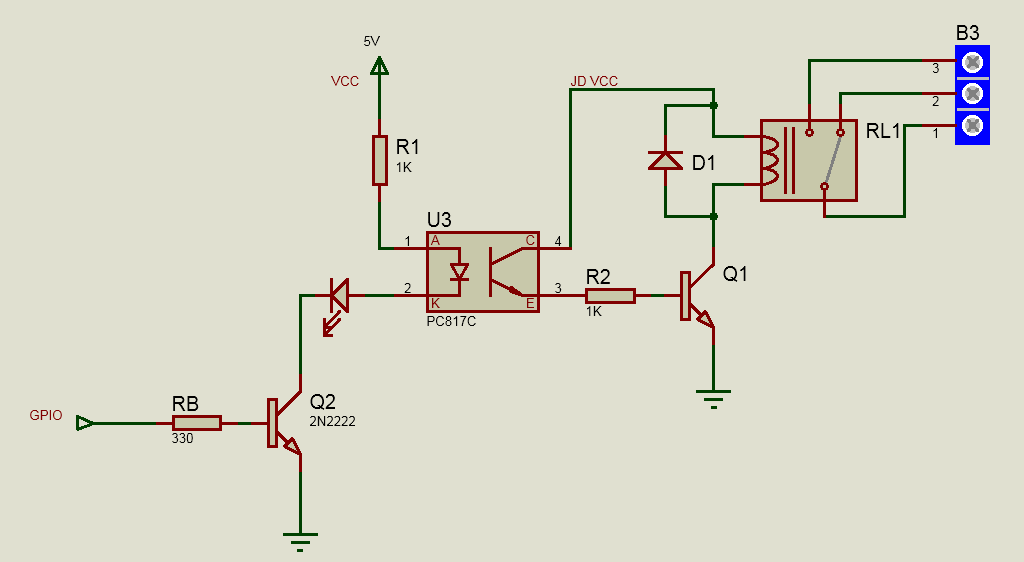
\includegraphics[width=13cm]{./img/composants/relaiset2n2222.PNG}
	\caption{Schéma du relais avec le transistor 2N2222}
	\label{fig:relais_5vdc}
\end{figure}

D’après la datasheet du transistor 2N2222 :
\begin{itemize}
	\item La tension de collecteur-émetteur en saturation (\(V_{CE_{sat}}\)) est d'environ 400 mV.
	\item Le gain minimal du transistor (\(\beta\)) est de 10.
\end{itemize}

D’après les caractéristiques du relais SONGLE SRD-05V DC SL-C :
\begin{itemize}
	\item La résistance de la bobine du relais est de 70 \(\Omega\).
	\item Alimenté par une tension \(V_{bobine} = V_{CC} - V_{CE_{sat}} = 5V - 0.4V = 4.6V\), le courant de collecteur (\(I_C\)) est donné par :
\end{itemize}

\[
I_C = \frac{V_{bobine}}{R_{bobine}} = \frac{4.6V}{70\Omega} = 0.0657A \approx 70mA
\]

Pour que le transistor fonctionne en mode commutation, il doit être saturé. Le courant de base (\(I_B\)) nécessaire est :

\[
I_B = \frac{I_C}{\beta} = \frac{70mA}{10} = 7mA
\]

La résistance de base (\(R_B\)) est calculée à partir de la tension de sortie de l'ESP32 (\(V_{GPIO}\)) et la tension de base-émetteur en saturation (\(V_{BE_{sat}}\)) du transistor :

\[
R_B = \frac{V_{GPIO} - V_{BE_{sat}}}{I_B}
\]

Avec \(V_{GPIO} = 3.3V\) et \(V_{BE_{sat}} = 0.8V\) :

\[
R_B = \frac{3.3V - 0.8V}{7mA} = \frac{2.5V}{0.007A} = 357.14 \Omega
\]

En utilisant une valeur normalisée disponible dans les séries de résistances (série E24), nous choisissons :

\[
R_B = 330 \Omega
\]
\subsubsection*{Diviseurs de tension et diode Zener 1N4728A}

Des diviseurs de tension sont utilisés pour abaisser la tension mesurée d'une batterie de 12V, qui peut atteindre jusqu'à 14.5V lorsqu'elle est complètement chargée, à des niveaux compatibles avec les entrées de l'ESP32 (3.3V). Chaque diviseur de tension est équipé d'une diode Zener 1N4728A pour protéger le microcontrôleur contre les surtensions en limitant la tension maximale appliquée aux broches de l'ESP32.

\subsubsection*{Calcul des résistances pour le diviseur de tension}
\begin{figure}[H]
	\centering
	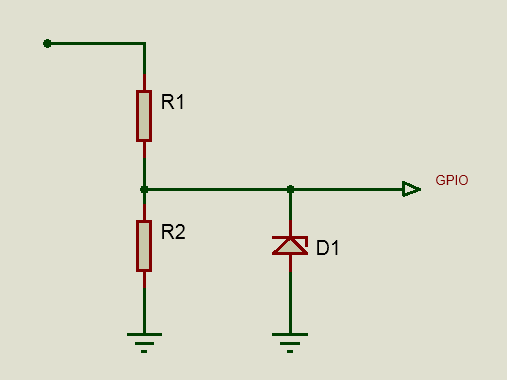
\includegraphics[width=6cm]{./img/composants/ddt.PNG}
	\caption{Schéma du diviseur de tension avec la diode zener 1N4728A}
	\label{fig:relais_5vdc}
\end{figure}

Pour réduire une tension d'entrée de 14.5V à une tension de sortie de 3V, les valeurs des résistances du diviseur de tension sont calculées comme suit :

\[
V_{s} = V_{e} \times \frac{R_2}{R_1 + R_2}
\]

où \( V_{e} = 14.5V \) et \( V_{s} = 3V \). 

Le rapport de résistances nécessaire est :

\[
\frac{R_2}{R_1 + R_2} = \frac{V_{s}}{V_{e}} = \frac{3V}{14.5V} \approx 0.2069
\]

En choisissant \( R_1 = 4 k\Omega \) et \( R_2 = 1 k\Omega \), nous calculons la tension de sortie comme suit :

\[
V_{s} = 14.5V \times \frac{1 k\Omega}{4 k\Omega + 1 k\Omega}
\]

\[
V_{s} = 14.5V \times \frac{1}{5} = 14.5V \times 0.2 = 2.9V
\]

Avec ces valeurs, la tension de sortie est d'environ 2.9V, proche de la cible de 3V. Ce choix facilite les calculs et offre une marge de sécurité supplémentaire. En optant pour 3V au lieu de 3.3V, nous simplifions l'utilisation de résistances standards et protégeons le microcontrôleur ESP32 contre les surtensions potentielles.

\subsubsection*{Capteurs ACS712 et diviseur de tension}

Les capteurs ACS712 mesurent le courant de charge et de décharge des batteries, et leur signal de sortie doit être adapté pour correspondre à l'entrée analogique de l'ESP32. Pour ce faire, nous utilisons des diviseurs de tension.

Supposons que la sortie maximale du capteur ACS712 soit de 5V. Nous souhaitons abaisser cette tension à un niveau compatible avec l'entrée analogique de l'ESP32, qui est de 3.3V. Le choix d'une tension de sortie légèrement inférieure à 3.3V (par exemple 3V) permet d'ajouter une marge de sécurité pour protéger l'ESP32.
\begin{figure}[H]
	\centering
	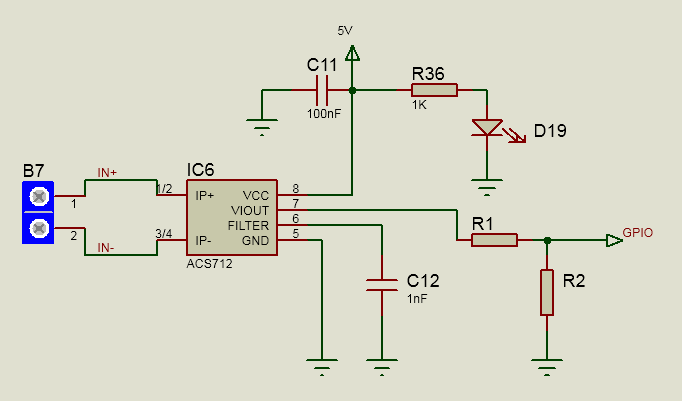
\includegraphics[width=13cm]{./img/composants/ACSAVECRESISTANCE.PNG}
	\caption{Schéma du ACS712 avec le diviseur de tension}
	\label{fig:relais_5vdc}
\end{figure}

Le rapport de résistance nécessaire est calculé comme suit :

\[
\frac{R_2}{R_1 + R_2} = \frac{V_{s}}{V_{e}} = \frac{3V}{5V} = 0.6
\]

Pour atteindre ce rapport avec des valeurs standard de résistances, nous choisissons \( R_1 \) et \( R_2 \). Supposons que nous choisissons \( R_2 = 2k\Omega \). Nous pouvons alors calculer \( R_1 \) en utilisant la formule :

\[
\frac{R_2}{R_1 + R_2} = 0.6 \implies R_1 + R_2 = \frac{R_2}{0.6}
\]

\[
R_1 = \frac{R_2}{0.6} - R_2 = \frac{2k\Omega}{0.6} - 2k\Omega = \frac{2000}{0.6} - 2000 \approx 3333 - 2000 = 1333 \Omega
\]

Nous choisissons alors la valeur standard la plus proche, \( R_1 = 1k\Omega \), et recalculons la tension de sortie :

\[
V_{s} = V_{e} \times \frac{R_2}{R_1 + R_2} = 5V \times \frac{2k\Omega}{1k\Omega + 2k\Omega} = 5V \times \frac{2}{3} \approx 3.33V
\]

Cette tension est légèrement au-dessus de 3.3V, offrant ainsi une marge de sécurité. Les valeurs choisies permettent d'adapter efficacement le signal de sortie du capteur à l'entrée de l'ESP32 tout en utilisant des résistances standards facilement disponibles.

\subsubsection{Brochage des Composants}
\subsubsection*{Relais}
\begin{table}[H]
	\centering
	\caption{Brochage des Relais}
	\begin{tabular}{|p{4.5cm}|p{3.5cm}|p{2cm}|p{3.5cm}|}
		\hline
		\rule[0.5cm]{0cm}{0cm} \textbf{Relais} & \textbf{GND} & \textbf{VCC} & \textbf{IN} \\
		\hline
		\rule[0.5cm]{0cm}{0cm} Relais 1 & GND de l'ESP32 & 5V & GPIO 5 \\
		\hline
		\rule[0.5cm]{0cm}{0cm} Relais 2 & GND de l'ESP32 & 5V & GPIO 18 \\
		\hline
		\rule[0.5cm]{0cm}{0cm} Relais 3 & GND de l'ESP32 & 5V & GPIO 19 \\
		\hline
		\rule[0.5cm]{0cm}{0cm} Relais 4 & GND de l'ESP32 & 5V & GPIO 23 \\
		\hline
	\end{tabular}
\end{table}

\subsubsection*{Capteurs de Courant (ACS712)}

\begin{table}[H]
	\centering
	\caption{Brochage des Capteurs de Courant (ACS712)}
	\begin{tabular}{|p{5.5cm}|p{2cm}|p{3.5cm}|p{2.5cm}|}
		\hline
		\rule[0.5cm]{0cm}{0cm} \textbf{Capteur} & \textbf{VCC} & \textbf{GND} & \textbf{OUT} \\
		\hline
		\rule[0.5cm]{0cm}{0cm} ACS712 pour Batterie 1 & 5V & GND de l'ESP32 & GPIO 36 \\
		\hline
		\rule[0.5cm]{0cm}{0cm} ACS712 pour Batterie 2 & 5V & GND de l'ESP32 & GPIO 39 \\
		\hline
		\rule[0.5cm]{0cm}{0cm} ACS712 pour Batterie 3 & 5V & GND de l'ESP32 & GPIO 25 \\
		\hline
		\rule[0.5cm]{0cm}{0cm} ACS712 pour Courant Global & 5V & GND de l'ESP32 & GPIO 26 \\
		\hline
	\end{tabular}
\end{table}

\subsubsection*{Capteurs de Température (LM35)}

\begin{table}[H]
	\centering
	\caption{Brochage des Capteurs de Température (LM35)}
	\begin{tabular}{|p{4.5cm}|p{2cm}|p{3.5cm}|p{3.5cm}|}
		\hline
		\rule[0.5cm]{0cm}{0cm} \textbf{Capteur} & \textbf{VCC} & \textbf{GND} & \textbf{OUT} \\
		\hline
		\rule[0.5cm]{0cm}{0cm} LM35 pour Batterie 1 & 5V & GND de l'ESP32 & GPIO 34 \\
		\hline
		\rule[0.5cm]{0cm}{0cm} LM35 pour Batterie 2 & 5V & GND de l'ESP32 & GPIO 35 \\
		\hline
		\rule[0.5cm]{0cm}{0cm} LM35 pour Batterie 3 & 5V & GND de l'ESP32 & GPIO 32 \\
		\hline
	\end{tabular}
\end{table}

\subsubsection*{Diviseurs de Tension}

\begin{table}[H]
	\centering
	\caption{Brochage des Diviseurs de Tension}
	\begin{tabular}{|p{6.5cm}|p{1.5cm}|p{3.5cm}|p{2cm}|}
		\hline
		\rule[0.5cm]{0cm}{0cm} \textbf{Diviseur de Tension} & \textbf{VCC} & \textbf{GND} & \textbf{OUT} \\
		\hline
		\rule[0.5cm]{0cm}{0cm} Diviseur de Tension pour Batterie 1 & 12V & GND de l'ESP32 & GPIO 33 \\
		\hline
		\rule[0.5cm]{0cm}{0cm} Diviseur de Tension pour Batterie 2 & 12V & GND de l'ESP32 & GPIO 27 \\
		\hline
		\rule[0.5cm]{0cm}{0cm} Diviseur de Tension pour Batterie 3 & 12V & GND de l'ESP32 & GPIO 14 \\
		\hline
		\rule[0.5cm]{0cm}{0cm} Diviseur de Tension pour Batterie Globale & 12V & GND de l'ESP32 & GPIO 12 \\
		\hline
	\end{tabular}
\end{table}

\subsubsection*{Afficheur LCD I2C}

\begin{table}[H]
	\centering
	\caption{Brochage de l'Afficheur LCD I2C}
	\begin{tabular}{|p{4.5cm}|p{2cm}|p{3cm}|p{2cm}|p{2cm}|}
		\hline
		\rule[0.5cm]{0cm}{0cm} \textbf{Afficheur LCD I2C} & \textbf{VCC} & \textbf{GND} & \textbf{SDA} & \textbf{SCL} \\
		\hline
		\rule[0.5cm]{0cm}{0cm} Afficheur LCD I2C & 5V & GND de l'ESP32 & GPIO 21 & GPIO 22 \\
		\hline
	\end{tabular}
\end{table}

\subsubsection*{Module GSM}

\begin{table}[H]
	\centering
	\caption{Brochage du Module GSM}
	\begin{tabular}{|p{4.5cm}|p{2cm}|p{3cm}|p{2cm}|p{2cm}|}
		\hline
		\rule[0.5cm]{0cm}{0cm} \textbf{Module GSM} & \textbf{VCC} & \textbf{GND} & \textbf{RX} & \textbf{TX} \\
		\hline
		\rule[0.5cm]{0cm}{0cm} Module GSM & 5V & GND de l'ESP32 & GPIO 17 & GPIO 16 \\
		\hline
	\end{tabular}
\end{table}

\subsubsection*{Leds}
\begin{table}[H]
	\centering
	\caption{Brochage des leds}
	\begin{tabular}{|p{4.5cm}|p{3.5cm}|p{3.5cm}|}
		\hline
		\rule[0.5cm]{0cm}{0cm} \textbf{Led} & \textbf{GND} & \textbf{OUT} \\
		\hline
		\rule[0.5cm]{0cm}{0cm} Led pour le gsm 1 & GND de l'ESP32  & GPIO 4 \\
		\hline
	\end{tabular}
\end{table}


\begin{landscape}
\begin{figure}[]
	\centering
	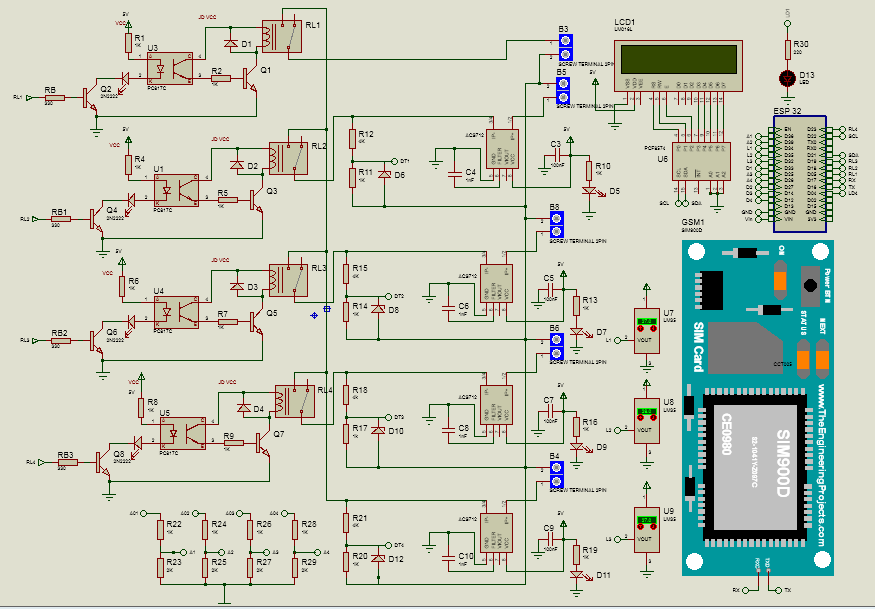
\includegraphics[width=25cm]{./img/schema22.PNG}
	\caption{Schéma d'ensemble du système}
	\label{fig:relais_5vdc}
\end{figure}
\end{landscape}

\subsection{Câblage réalisé}
Tous les composants électroniques ont été montés et soudés sur une plaquette perforée à l'aide de fil bobine pour les liaisons. Seuls les capteurs de température nécessitent l'utilisation de connecteurs USB mâles/femelles pour assurer leur connexion avec le dispositif, tandis que les capteurs de tension et de courant sont directement reliés au système de surveillance des batteries solaires.

\begin{figure}[H]
	\centering
	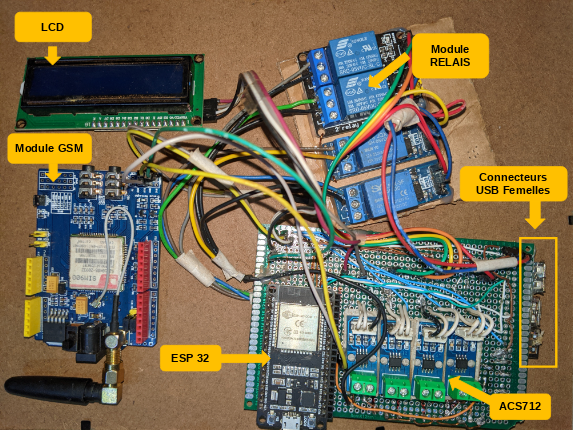
\includegraphics[width=10cm]{./img/composants/realisation.png}

	\label{fig:relais_5vdc}
\end{figure}
\begin{figure}[H]
	\centering
	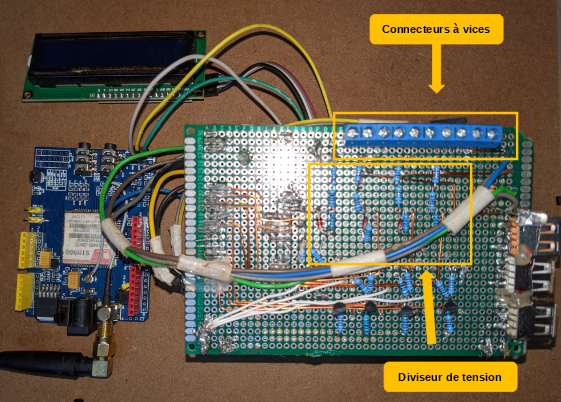
\includegraphics[width=10cm]{./img/composants/realisationDos.png}
		\caption{Câblage des composantes}
	\label{fig:relais_5vdc}
\end{figure}

\subsection{Mise en boîte}
Dimensionner et concevoir le boîtier afin d'accueillir les composants déjà câblés, notamment le port USB femelle, l'écran LCD, l'antenne, la puce GSM, les LED et les fixations des fils reliés aux batteries, tout en prenant en compte les contraintes de taille et d'accessibilité pour une utilisation optimale.

\begin{figure}[H]
	\centering
	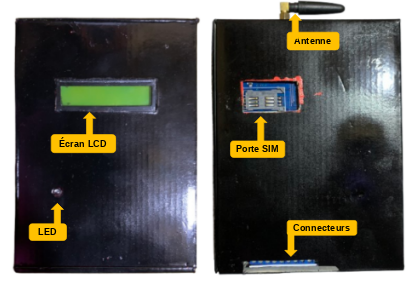
\includegraphics[width=17cm]{./img/dispo3.png}
\caption{Mise en boîte du dispositif}
\end{figure}
\begin{figure}[H]
	\centering
	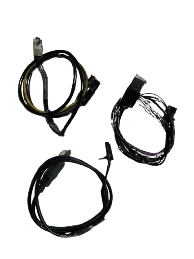
\includegraphics[width=4cm]{./img/cable.png}
\caption{Câbles avec connecteur USB mâle pour les capteurs LM35}

\end{figure}

\section{Conclusion}

Ce chapitre a permis d'explorer le dimensionnement des composants essentiels en calculant leurs valeurs, ainsi que d'examiner les interfaces de puissance et les brochages entre le microcontrôleur ESP32 et les autres composants qui lui sont reliés. La présentation du câblage a illustré comment chaque élément s'assemble pour former un système cohérent et fonctionnel. Ces connaissances constituent une base solide pour les étapes suivantes de notre projet, y compris la réalisation du tableau de bord, ainsi que l'implémentation et les tests.

